% Options for packages loaded elsewhere
\PassOptionsToPackage{unicode}{hyperref}
\PassOptionsToPackage{hyphens}{url}
%
\documentclass[
]{article}
\usepackage{amsmath,amssymb}
\usepackage{iftex}
\ifPDFTeX
  \usepackage[T1]{fontenc}
  \usepackage[utf8]{inputenc}
  \usepackage{textcomp} % provide euro and other symbols
\else % if luatex or xetex
  \usepackage{unicode-math} % this also loads fontspec
  \defaultfontfeatures{Scale=MatchLowercase}
  \defaultfontfeatures[\rmfamily]{Ligatures=TeX,Scale=1}
\fi
\usepackage{lmodern}
\ifPDFTeX\else
  % xetex/luatex font selection
\fi
% Use upquote if available, for straight quotes in verbatim environments
\IfFileExists{upquote.sty}{\usepackage{upquote}}{}
\IfFileExists{microtype.sty}{% use microtype if available
  \usepackage[]{microtype}
  \UseMicrotypeSet[protrusion]{basicmath} % disable protrusion for tt fonts
}{}
\makeatletter
\@ifundefined{KOMAClassName}{% if non-KOMA class
  \IfFileExists{parskip.sty}{%
    \usepackage{parskip}
  }{% else
    \setlength{\parindent}{0pt}
    \setlength{\parskip}{6pt plus 2pt minus 1pt}}
}{% if KOMA class
  \KOMAoptions{parskip=half}}
\makeatother
\usepackage{xcolor}
\usepackage[margin=1in]{geometry}
\usepackage{color}
\usepackage{fancyvrb}
\newcommand{\VerbBar}{|}
\newcommand{\VERB}{\Verb[commandchars=\\\{\}]}
\DefineVerbatimEnvironment{Highlighting}{Verbatim}{commandchars=\\\{\}}
% Add ',fontsize=\small' for more characters per line
\usepackage{framed}
\definecolor{shadecolor}{RGB}{248,248,248}
\newenvironment{Shaded}{\begin{snugshade}}{\end{snugshade}}
\newcommand{\AlertTok}[1]{\textcolor[rgb]{0.94,0.16,0.16}{#1}}
\newcommand{\AnnotationTok}[1]{\textcolor[rgb]{0.56,0.35,0.01}{\textbf{\textit{#1}}}}
\newcommand{\AttributeTok}[1]{\textcolor[rgb]{0.13,0.29,0.53}{#1}}
\newcommand{\BaseNTok}[1]{\textcolor[rgb]{0.00,0.00,0.81}{#1}}
\newcommand{\BuiltInTok}[1]{#1}
\newcommand{\CharTok}[1]{\textcolor[rgb]{0.31,0.60,0.02}{#1}}
\newcommand{\CommentTok}[1]{\textcolor[rgb]{0.56,0.35,0.01}{\textit{#1}}}
\newcommand{\CommentVarTok}[1]{\textcolor[rgb]{0.56,0.35,0.01}{\textbf{\textit{#1}}}}
\newcommand{\ConstantTok}[1]{\textcolor[rgb]{0.56,0.35,0.01}{#1}}
\newcommand{\ControlFlowTok}[1]{\textcolor[rgb]{0.13,0.29,0.53}{\textbf{#1}}}
\newcommand{\DataTypeTok}[1]{\textcolor[rgb]{0.13,0.29,0.53}{#1}}
\newcommand{\DecValTok}[1]{\textcolor[rgb]{0.00,0.00,0.81}{#1}}
\newcommand{\DocumentationTok}[1]{\textcolor[rgb]{0.56,0.35,0.01}{\textbf{\textit{#1}}}}
\newcommand{\ErrorTok}[1]{\textcolor[rgb]{0.64,0.00,0.00}{\textbf{#1}}}
\newcommand{\ExtensionTok}[1]{#1}
\newcommand{\FloatTok}[1]{\textcolor[rgb]{0.00,0.00,0.81}{#1}}
\newcommand{\FunctionTok}[1]{\textcolor[rgb]{0.13,0.29,0.53}{\textbf{#1}}}
\newcommand{\ImportTok}[1]{#1}
\newcommand{\InformationTok}[1]{\textcolor[rgb]{0.56,0.35,0.01}{\textbf{\textit{#1}}}}
\newcommand{\KeywordTok}[1]{\textcolor[rgb]{0.13,0.29,0.53}{\textbf{#1}}}
\newcommand{\NormalTok}[1]{#1}
\newcommand{\OperatorTok}[1]{\textcolor[rgb]{0.81,0.36,0.00}{\textbf{#1}}}
\newcommand{\OtherTok}[1]{\textcolor[rgb]{0.56,0.35,0.01}{#1}}
\newcommand{\PreprocessorTok}[1]{\textcolor[rgb]{0.56,0.35,0.01}{\textit{#1}}}
\newcommand{\RegionMarkerTok}[1]{#1}
\newcommand{\SpecialCharTok}[1]{\textcolor[rgb]{0.81,0.36,0.00}{\textbf{#1}}}
\newcommand{\SpecialStringTok}[1]{\textcolor[rgb]{0.31,0.60,0.02}{#1}}
\newcommand{\StringTok}[1]{\textcolor[rgb]{0.31,0.60,0.02}{#1}}
\newcommand{\VariableTok}[1]{\textcolor[rgb]{0.00,0.00,0.00}{#1}}
\newcommand{\VerbatimStringTok}[1]{\textcolor[rgb]{0.31,0.60,0.02}{#1}}
\newcommand{\WarningTok}[1]{\textcolor[rgb]{0.56,0.35,0.01}{\textbf{\textit{#1}}}}
\usepackage{graphicx}
\makeatletter
\def\maxwidth{\ifdim\Gin@nat@width>\linewidth\linewidth\else\Gin@nat@width\fi}
\def\maxheight{\ifdim\Gin@nat@height>\textheight\textheight\else\Gin@nat@height\fi}
\makeatother
% Scale images if necessary, so that they will not overflow the page
% margins by default, and it is still possible to overwrite the defaults
% using explicit options in \includegraphics[width, height, ...]{}
\setkeys{Gin}{width=\maxwidth,height=\maxheight,keepaspectratio}
% Set default figure placement to htbp
\makeatletter
\def\fps@figure{htbp}
\makeatother
\setlength{\emergencystretch}{3em} % prevent overfull lines
\providecommand{\tightlist}{%
  \setlength{\itemsep}{0pt}\setlength{\parskip}{0pt}}
\setcounter{secnumdepth}{-\maxdimen} % remove section numbering
\ifLuaTeX
  \usepackage{selnolig}  % disable illegal ligatures
\fi
\IfFileExists{bookmark.sty}{\usepackage{bookmark}}{\usepackage{hyperref}}
\IfFileExists{xurl.sty}{\usepackage{xurl}}{} % add URL line breaks if available
\urlstyle{same}
\hypersetup{
  pdftitle={HUDM6052 Psychometric II Homework\_03},
  pdfauthor={Chenguang Pan (cp3280@tc.columbia.edu)},
  hidelinks,
  pdfcreator={LaTeX via pandoc}}

\title{HUDM6052 Psychometric II Homework\_03}
\author{Chenguang Pan
(\href{mailto:cp3280@tc.columbia.edu}{\nolinkurl{cp3280@tc.columbia.edu}})}
\date{2023-10-26}

\begin{document}
\maketitle

\setcounter{tocdepth}{4}
\tableofcontents

\hypertarget{q1}{%
\subsection{Q1}\label{q1}}

\emph{Using the item parameters given in the Table\ldots{}}

\textbf{My Solution:}

\begin{Shaded}
\begin{Highlighting}[]
\SpecialCharTok{\textgreater{}} \CommentTok{\# write the corresponding information function}
\ErrorTok{\textgreater{}}\NormalTok{ iif }\OtherTok{\textless{}{-}} \ControlFlowTok{function}\NormalTok{(theta, a, b)\{}
\SpecialCharTok{+}   \CommentTok{\# get the logit}
\SpecialCharTok{+}\NormalTok{   Z }\OtherTok{\textless{}{-}}\NormalTok{ a}\SpecialCharTok{*}\NormalTok{(theta}\SpecialCharTok{{-}}\NormalTok{b)}
\SpecialCharTok{+}   \CommentTok{\# get the probability}
\SpecialCharTok{+}\NormalTok{   out }\OtherTok{\textless{}{-}} \DecValTok{1}\SpecialCharTok{/}\NormalTok{(}\DecValTok{1} \SpecialCharTok{+} \FunctionTok{exp}\NormalTok{(}\SpecialCharTok{{-}}\NormalTok{Z))}
\SpecialCharTok{+}\NormalTok{   info }\OtherTok{\textless{}{-}}\NormalTok{ out}\SpecialCharTok{*}\NormalTok{(}\DecValTok{1}\SpecialCharTok{{-}}\NormalTok{out)}\SpecialCharTok{*}\NormalTok{(a}\SpecialCharTok{\^{}}\DecValTok{2}\NormalTok{)}
\SpecialCharTok{+}   \FunctionTok{return}\NormalTok{(info)}
\SpecialCharTok{+}\NormalTok{ \}}
\SpecialCharTok{\textgreater{}} 
\ErrorTok{\textgreater{}} \CommentTok{\# set the ability range}
\ErrorTok{\textgreater{}}\NormalTok{ theta }\OtherTok{\textless{}{-}} \FunctionTok{seq}\NormalTok{(}\SpecialCharTok{{-}}\DecValTok{3}\NormalTok{,}\DecValTok{3}\NormalTok{, }\AttributeTok{by=}\FloatTok{0.5}\NormalTok{)}
\SpecialCharTok{\textgreater{}} \CommentTok{\# set the item parameters}
\ErrorTok{\textgreater{}}\NormalTok{ a }\OtherTok{\textless{}{-}} \FunctionTok{c}\NormalTok{(}\DecValTok{2}\NormalTok{, }\FloatTok{1.5}\NormalTok{, }\FloatTok{1.5}\NormalTok{, }\FloatTok{1.5}\NormalTok{, }\DecValTok{2}\NormalTok{)}
\SpecialCharTok{\textgreater{}}\NormalTok{ b }\OtherTok{\textless{}{-}} \FunctionTok{c}\NormalTok{(}\SpecialCharTok{{-}}\DecValTok{1}\NormalTok{, }\SpecialCharTok{{-}}\FloatTok{0.5}\NormalTok{, }\DecValTok{0}\NormalTok{, }\FloatTok{0.5}\NormalTok{, }\DecValTok{1}\NormalTok{)}
\SpecialCharTok{\textgreater{}} \CommentTok{\# define the color}
\ErrorTok{\textgreater{}}\NormalTok{ color\_set }\OtherTok{\textless{}{-}} \FunctionTok{c}\NormalTok{(}\StringTok{"red"}\NormalTok{, }\StringTok{"green"}\NormalTok{, }\StringTok{"blue"}\NormalTok{,}\StringTok{"violet"}\NormalTok{,}\StringTok{"black"}\NormalTok{)}
\SpecialCharTok{\textgreater{}} 
\ErrorTok{\textgreater{}} \CommentTok{\# plot the item information function}
\ErrorTok{\textgreater{}}\NormalTok{ info\_out }\OtherTok{\textless{}{-}} \FunctionTok{iif}\NormalTok{(theta, a[}\DecValTok{1}\NormalTok{], b[}\DecValTok{1}\NormalTok{])}
\SpecialCharTok{\textgreater{}} \CommentTok{\# create a vector to sum up all the information function}
\ErrorTok{\textgreater{}}\NormalTok{ test\_info }\OtherTok{\textless{}{-}}\NormalTok{ info\_out}
\SpecialCharTok{\textgreater{}} 
\ErrorTok{\textgreater{}} \CommentTok{\# initialize the plot by plotting the first item}
\ErrorTok{\textgreater{}} \FunctionTok{plot}\NormalTok{(theta, info\_out,}\AttributeTok{type =} \StringTok{"l"}\NormalTok{, }\AttributeTok{col=}\NormalTok{color\_set[}\DecValTok{1}\NormalTok{],}
\SpecialCharTok{+}      \AttributeTok{main =} \StringTok{"Item/Test Information and SEs"}\NormalTok{,}
\SpecialCharTok{+}      \AttributeTok{xlab =} \StringTok{"Ability"}\NormalTok{, }\AttributeTok{ylab =} \StringTok{"information"}\NormalTok{,}
\SpecialCharTok{+}      \AttributeTok{ylim =} \FunctionTok{c}\NormalTok{(}\DecValTok{0}\NormalTok{,}\DecValTok{3}\NormalTok{))}
\SpecialCharTok{\textgreater{}} \FunctionTok{grid}\NormalTok{()}
\SpecialCharTok{\textgreater{}} 
\ErrorTok{\textgreater{}} \CommentTok{\# plot the rest item using a for loop}
\ErrorTok{\textgreater{}} \ControlFlowTok{for}\NormalTok{ (i }\ControlFlowTok{in} \DecValTok{2}\SpecialCharTok{:}\DecValTok{5}\NormalTok{) \{}
\SpecialCharTok{+}\NormalTok{   info\_out\_i }\OtherTok{\textless{}{-}} \FunctionTok{iif}\NormalTok{(theta,a[i],b[i])}
\SpecialCharTok{+}   \FunctionTok{lines}\NormalTok{(theta, info\_out\_i, }\AttributeTok{type =}\StringTok{"l"}\NormalTok{, }\AttributeTok{col=}\NormalTok{color\_set[i])}
\SpecialCharTok{+}\NormalTok{   test\_info }\OtherTok{\textless{}{-}}\NormalTok{ test\_info }\SpecialCharTok{+}\NormalTok{info\_out\_i}
\SpecialCharTok{+}\NormalTok{ \}}
\SpecialCharTok{\textgreater{}} 
\ErrorTok{\textgreater{}} \CommentTok{\# draw the test information function}
\ErrorTok{\textgreater{}} \FunctionTok{lines}\NormalTok{(theta, test\_info, }\AttributeTok{type =} \StringTok{"l"}\NormalTok{, }\AttributeTok{col=}\StringTok{"gray"}\NormalTok{)}
\SpecialCharTok{\textgreater{}} \CommentTok{\# plot the SE }
\ErrorTok{\textgreater{}}\NormalTok{ SE }\OtherTok{\textless{}{-}} \FunctionTok{c}\NormalTok{()}
\SpecialCharTok{\textgreater{}} \ControlFlowTok{for}\NormalTok{ (j }\ControlFlowTok{in} \DecValTok{1}\SpecialCharTok{:}\FunctionTok{length}\NormalTok{(theta)) \{}
\SpecialCharTok{+}\NormalTok{   se\_j }\OtherTok{\textless{}{-}} \DecValTok{1}\SpecialCharTok{/}\FunctionTok{sqrt}\NormalTok{(}\FunctionTok{sum}\NormalTok{(}\FunctionTok{iif}\NormalTok{(theta[j],a,b)))}
\SpecialCharTok{+}\NormalTok{   SE[j] }\OtherTok{\textless{}{-}}\NormalTok{ se\_j}
\SpecialCharTok{+}\NormalTok{ \}}
\SpecialCharTok{\textgreater{}} \FunctionTok{lines}\NormalTok{(theta, SE, }\AttributeTok{type =} \StringTok{"l"}\NormalTok{, }\AttributeTok{col=}\StringTok{"pink"}\NormalTok{)}
\SpecialCharTok{\textgreater{}} 
\ErrorTok{\textgreater{}} \CommentTok{\# add a legend}
\ErrorTok{\textgreater{}} \FunctionTok{legend}\NormalTok{(}\StringTok{\textquotesingle{}topright\textquotesingle{}}\NormalTok{,}\AttributeTok{inset=}\FloatTok{0.05}\NormalTok{,}\FunctionTok{c}\NormalTok{(}\StringTok{"item 1"}\NormalTok{,}\StringTok{"item 2"}\NormalTok{,}\StringTok{"item 3"}\NormalTok{,}\StringTok{"item 4"}\NormalTok{,}\StringTok{"item 5"}\NormalTok{,}
\SpecialCharTok{+}                               \StringTok{"test information"}\NormalTok{,}\StringTok{"SE"}\NormalTok{),}
\SpecialCharTok{+}        \AttributeTok{lty=}\DecValTok{1}\NormalTok{,}\AttributeTok{col=}\FunctionTok{c}\NormalTok{(}\StringTok{"red"}\NormalTok{, }\StringTok{"green"}\NormalTok{,}\StringTok{"blue"}\NormalTok{,}\StringTok{"violet"}\NormalTok{,}\StringTok{"black"}\NormalTok{,}\StringTok{"gray"}\NormalTok{,}\StringTok{"pink"}\NormalTok{),}
\SpecialCharTok{+}        \AttributeTok{title=}\StringTok{"Line Type"}\NormalTok{, }\AttributeTok{cex =} \FloatTok{0.5}\NormalTok{)}
\end{Highlighting}
\end{Shaded}

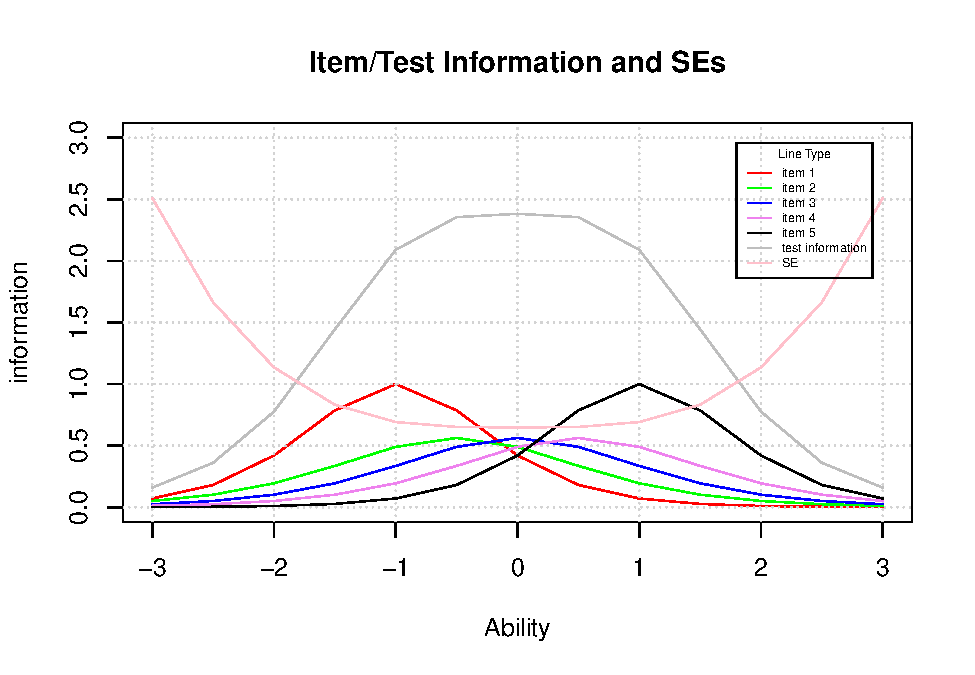
\includegraphics{Assignment_3_files/figure-latex/unnamed-chunk-1-1.pdf}

\hypertarget{q2.a}{%
\subsection{Q2.a}\label{q2.a}}

\emph{a. For each of the six items given in the Table below\ldots{}}

\textbf{My Solution:}\\
The maximum value of a 3PL's information function is at
\[\theta_{max}=\beta_i + \frac{1}{a_i}log[\frac{1+\sqrt{1+8c_i}}{2}].\]\\
Therefore, I write a function to get the optimal \(\theta_{max}\) first.
And then send this value together with the parameters into the
information function for 3PL model to get the results.

\begin{Shaded}
\begin{Highlighting}[]
\SpecialCharTok{\textgreater{}} \CommentTok{\# write a function to get the theta\_max}
\ErrorTok{\textgreater{}}\NormalTok{ get\_theta }\OtherTok{\textless{}{-}} \ControlFlowTok{function}\NormalTok{(a,b,c)\{}
\SpecialCharTok{+}\NormalTok{   out }\OtherTok{\textless{}{-}}\NormalTok{ b }\SpecialCharTok{+} \FunctionTok{log}\NormalTok{(}\FloatTok{0.5+0.5}\SpecialCharTok{*}\FunctionTok{sqrt}\NormalTok{(}\DecValTok{1}\SpecialCharTok{+}\DecValTok{8}\SpecialCharTok{*}\NormalTok{c))}\SpecialCharTok{/}\NormalTok{a}
\SpecialCharTok{+}   \FunctionTok{return}\NormalTok{(out)}
\SpecialCharTok{+}\NormalTok{ \}}
\SpecialCharTok{\textgreater{}} 
\ErrorTok{\textgreater{}} \CommentTok{\# write the 3pl information function}
\ErrorTok{\textgreater{}}\NormalTok{ iif\_3pl }\OtherTok{\textless{}{-}} \ControlFlowTok{function}\NormalTok{(theta, a, b, c)\{}
\SpecialCharTok{+}\NormalTok{   z }\OtherTok{\textless{}{-}}\NormalTok{ a}\SpecialCharTok{*}\NormalTok{(theta }\SpecialCharTok{{-}}\NormalTok{ b)}
\SpecialCharTok{+}\NormalTok{   p }\OtherTok{\textless{}{-}}\NormalTok{ c }\SpecialCharTok{+}\NormalTok{ (}\DecValTok{1}\SpecialCharTok{{-}}\NormalTok{c)}\SpecialCharTok{/}\NormalTok{(}\DecValTok{1}\SpecialCharTok{+}\FunctionTok{exp}\NormalTok{(}\SpecialCharTok{{-}}\NormalTok{z))}
\SpecialCharTok{+}\NormalTok{   p\_star }\OtherTok{\textless{}{-}} \DecValTok{1}\SpecialCharTok{/}\NormalTok{(}\DecValTok{1} \SpecialCharTok{+} \FunctionTok{exp}\NormalTok{(}\SpecialCharTok{{-}}\NormalTok{z))}
\SpecialCharTok{+}\NormalTok{   I }\OtherTok{\textless{}{-}}\NormalTok{ (a}\SpecialCharTok{\^{}}\DecValTok{2}\NormalTok{)}\SpecialCharTok{*}\NormalTok{p}\SpecialCharTok{*}\NormalTok{(}\DecValTok{1}\SpecialCharTok{{-}}\NormalTok{p)}\SpecialCharTok{*}\NormalTok{(p\_star}\SpecialCharTok{/}\NormalTok{p)}\SpecialCharTok{\^{}}\DecValTok{2}
\SpecialCharTok{+}   \FunctionTok{return}\NormalTok{(I)}
\SpecialCharTok{+}\NormalTok{ \}}
\end{Highlighting}
\end{Shaded}

Next, plug the given paramters into the functions to get the results.

\begin{Shaded}
\begin{Highlighting}[]
\SpecialCharTok{\textgreater{}} \CommentTok{\# load the given parameters vectors}
\ErrorTok{\textgreater{}}\NormalTok{ b }\OtherTok{\textless{}{-}} \FunctionTok{c}\NormalTok{(}\DecValTok{1}\NormalTok{,}\DecValTok{1}\NormalTok{,}\DecValTok{1}\NormalTok{,}\SpecialCharTok{{-}}\FloatTok{1.5}\NormalTok{,}\SpecialCharTok{{-}}\FloatTok{0.5}\NormalTok{,}\FloatTok{0.5}\NormalTok{)}
\SpecialCharTok{\textgreater{}}\NormalTok{ a }\OtherTok{\textless{}{-}} \FunctionTok{c}\NormalTok{(}\FloatTok{1.8}\NormalTok{,}\FloatTok{0.8}\NormalTok{,}\FloatTok{1.8}\NormalTok{,}\FloatTok{1.8}\NormalTok{,}\FloatTok{1.2}\NormalTok{,}\FloatTok{0.4}\NormalTok{)}
\SpecialCharTok{\textgreater{}}\NormalTok{ c }\OtherTok{\textless{}{-}} \FunctionTok{c}\NormalTok{(}\DecValTok{0}\NormalTok{,}\DecValTok{0}\NormalTok{,}\FloatTok{0.25}\NormalTok{,}\DecValTok{0}\NormalTok{,}\FloatTok{0.1}\NormalTok{,}\FloatTok{0.15}\NormalTok{)}
\SpecialCharTok{\textgreater{}} 
\ErrorTok{\textgreater{}} \CommentTok{\# using a for loop to get all the required values}
\ErrorTok{\textgreater{}}\NormalTok{ theta\_vec }\OtherTok{\textless{}{-}} \FunctionTok{c}\NormalTok{()}
\SpecialCharTok{\textgreater{}}\NormalTok{ info\_vec }\OtherTok{\textless{}{-}} \FunctionTok{c}\NormalTok{()}
\SpecialCharTok{\textgreater{}} \ControlFlowTok{for}\NormalTok{ (i }\ControlFlowTok{in} \DecValTok{1}\SpecialCharTok{:}\FunctionTok{length}\NormalTok{(b)) \{}
\SpecialCharTok{+}   \CommentTok{\# get the optimal theta value}
\SpecialCharTok{+}\NormalTok{   theta\_max }\OtherTok{\textless{}{-}} \FunctionTok{get\_theta}\NormalTok{(}\AttributeTok{a =}\NormalTok{ a[i],}\AttributeTok{b =}\NormalTok{ b[i],}\AttributeTok{c =}\NormalTok{ c[i])}
\SpecialCharTok{+}\NormalTok{   theta\_vec[i] }\OtherTok{\textless{}{-}}\NormalTok{ theta\_max}
\SpecialCharTok{+}   \CommentTok{\# get the maximum value of information of item i}
\SpecialCharTok{+}\NormalTok{   info\_max }\OtherTok{\textless{}{-}} \FunctionTok{iif\_3pl}\NormalTok{(}\AttributeTok{theta =}\NormalTok{ theta\_max,}\AttributeTok{a =}\NormalTok{ a[i],}\AttributeTok{b =}\NormalTok{ b[i],}\AttributeTok{c =}\NormalTok{ c[i])}
\SpecialCharTok{+}\NormalTok{   info\_vec[i] }\OtherTok{\textless{}{-}}\NormalTok{ info\_max}
\SpecialCharTok{+}\NormalTok{ \}}
\SpecialCharTok{\textgreater{}} 
\ErrorTok{\textgreater{}} \CommentTok{\# Merge all the values as a dataframe}
\ErrorTok{\textgreater{}}\NormalTok{ df\_out }\OtherTok{\textless{}{-}} \FunctionTok{data.frame}\NormalTok{(}
\SpecialCharTok{+}   \AttributeTok{item =} \FunctionTok{seq}\NormalTok{(}\DecValTok{1}\NormalTok{,}\DecValTok{6}\NormalTok{),}
\SpecialCharTok{+}   \AttributeTok{theta\_max =}\NormalTok{ theta\_vec,}
\SpecialCharTok{+}   \AttributeTok{info\_max =}\NormalTok{ info\_vec}
\SpecialCharTok{+}\NormalTok{ )}
\SpecialCharTok{\textgreater{}} 
\ErrorTok{\textgreater{}}\NormalTok{ df\_out}
\NormalTok{  item  theta\_max   info\_max}
\DecValTok{1}    \DecValTok{1}  \FloatTok{1.0000000} \FloatTok{0.81000000}
\DecValTok{2}    \DecValTok{2}  \FloatTok{1.0000000} \FloatTok{0.16000000}
\DecValTok{3}    \DecValTok{3}  \FloatTok{1.1732808} \FloatTok{0.50122974}
\DecValTok{4}    \DecValTok{4} \SpecialCharTok{{-}}\FloatTok{1.5000000} \FloatTok{0.81000000}
\DecValTok{5}    \DecValTok{5} \SpecialCharTok{{-}}\FloatTok{0.3685794} \FloatTok{0.29665631}
\DecValTok{6}    \DecValTok{6}  \FloatTok{1.0410421} \FloatTok{0.02998276}
\end{Highlighting}
\end{Shaded}

The maximum values of information and corresponding \(\theta s\) are
shown at end of the code chunk above.

\hypertarget{q2.b}{%
\subsection{Q2.b}\label{q2.b}}

\emph{b. Which item would you choose to make up a two-item\ldots{}}

\textbf{My Solution:}\\
I will choose the \texttt{item\ 1} and \texttt{item\ 2} to make a
two-item test since they have the maximum information at the
\(\theta = 1.0\), which means this test can more accurately measure this
given test-taker's ability. The test information at \(\theta = 1.0\) is
\[0.81+0.16=0.97.\]

\hypertarget{q3}{%
\subsection{Q3}\label{q3}}

\emph{a. Determine the standard error of the estimate\ldots{}}

\textbf{My Solution:}

\begin{Shaded}
\begin{Highlighting}[]
\SpecialCharTok{\textgreater{}} \CommentTok{\# load the given paramters}
\ErrorTok{\textgreater{}}\NormalTok{ a }\OtherTok{\textless{}{-}} \FunctionTok{c}\NormalTok{(}\DecValTok{1}\NormalTok{,}\DecValTok{1}\NormalTok{,}\DecValTok{2}\NormalTok{,}\DecValTok{2}\NormalTok{)}
\SpecialCharTok{\textgreater{}}\NormalTok{ b }\OtherTok{\textless{}{-}} \FunctionTok{c}\NormalTok{(}\DecValTok{0}\NormalTok{,}\DecValTok{1}\NormalTok{,}\DecValTok{1}\NormalTok{,}\FloatTok{1.5}\NormalTok{)}
\SpecialCharTok{\textgreater{}}\NormalTok{ theta }\OtherTok{\textless{}{-}} \FloatTok{1.5}
\SpecialCharTok{\textgreater{}} 
\ErrorTok{\textgreater{}} \CommentTok{\# using the information function created in the Q1 to get the }
\ErrorTok{\textgreater{}} \CommentTok{\# vector of information at the theta=1.5 for each item}
\ErrorTok{\textgreater{}}\NormalTok{ info\_vec }\OtherTok{\textless{}{-}} \FunctionTok{iif}\NormalTok{(}\AttributeTok{theta=}\FloatTok{1.5}\NormalTok{, a, b)}
\SpecialCharTok{\textgreater{}} 
\ErrorTok{\textgreater{}} \CommentTok{\# get the SE}
\ErrorTok{\textgreater{}}\NormalTok{ SE\_j }\OtherTok{\textless{}{-}} \DecValTok{1}\SpecialCharTok{/}\FunctionTok{sqrt}\NormalTok{(}\FunctionTok{sum}\NormalTok{(info\_vec))}
\SpecialCharTok{\textgreater{}}\NormalTok{ SE\_j}
\NormalTok{[}\DecValTok{1}\NormalTok{] }\FloatTok{0.6787507}
\end{Highlighting}
\end{Shaded}

Therefore, the SE for the test-taker with estimated trait \(\theta=1.5\)
is 0.679.

\end{document}
